\chapter{音楽信号解析}

\begin{leadbox}
本章では,モノラル音楽音響信号の解析技術について解説します.
まず,音楽音響信号を音符単位に分解(音源分離・自動採譜)するうえで有用な
非負値行列因子分解 (nonnegative matrix factorization: NMF) および
確率的潜在成分解析 (probabilistic latent component analysis: PLCA) を説明します.
両手法ともに,ある確率モデルの最尤推定として解釈することが可能ですが,
NMFは階乗モデル (factorial model),PLCAは混合モデル (mixture model) に対応している点で異なります.
また,両手法ともに,これらの性質の違いを考慮した適切な事前分布を導入することにより,
ノンパラメトリックベイズモデルの定式化とベイズ推定が可能になります.
一方,音楽音響信号を異なる音響的性質をもつ音源信号に分解する技術についても解説します.
例えば,音楽音響信号を調波音と打楽器音に分離する技術,
歌声と伴奏音に分離する技術などが近年盛んに研究されています.

\end{leadbox}

\section{音楽音響信号の構成要素への分解}
\label{sec:introduction}

音楽情報処理においては,
解析対象となる音楽音響信号はモノラル(1チャネル)であることを想定するのが一般的です.
市販CDに録音されている音楽音響信号は,
ステレオ(左右2チャネル)形式であることがほとんどですが,
通常のマルチチャネル信号処理技術(\ref{sec:mic_array}章)は多くの場合使えません.
ポピュラー音楽の制作過程においては,
各楽器パートを別々のマイクで個別に録音しておき,
定位感を演出するために左右の音量バランスのみを調節してから,
全パートをミキシングすることが広く行われています.
この場合,各楽器パートのステレオ信号には,
実際に2つのマイクを楽器の前において録音した時とは異なり,
左右チャネルで位相差がありません.
本書では,左右チャネルの音量差に着目する音響信号解析手法は取り扱わず,
ステレオ信号はあらかじめモノラル信号に変換してから処理を行うものとします.

解析対象の情報を一切与えずに,すなわちブラインド環境下において,
モノラルの音楽音響信号を
構成要素に分解することは非常に難しい課題です.
ここで,何を構成要素とみなすべきかは,タスクに合わせて十分な検討が必要です.
例えば,自動採譜では,音楽音響信号を楽譜に変換することを目的としているため,
構成要素は音符に対応していることが望まれます.
一方,音楽音響信号を
歌声・ギター・ベース・ドラムといった楽器パートごとに分離したいのであれば,
構成要素は楽器音の音色に対応していなければなりません.
このように,構成要素 (parts) を定義すれば,
それらの組み合わせによって複雑な音楽音響信号が生成される過程を考えることにより,
独自の確率的生成モデルを定式化することができます(順問題).
いったん確率モデルが定式化できれば,
観測変数として音楽音響信号が与えられた時に,
潜在変数である構成要素や生成過程における各種のパラメータを
推定する問題を解くことが目標になります(逆問題).

モノラル音響信号の分離は数学的に不良設定問題(劣決定)であり,
なんらかの制約や基準なしでは最適解を一意に定めることができません.
簡単に言えば,$X+Y=10$を満たす$X$や$Y$を一意に定められないのと同じことで,
$X$や$Y$が満たすべき性質を適切に表現し,
その制約がどの程度満たされているかを数値化することにより,
はじめて最適な$X$や$Y$を求めることができます.
したがって,音楽音響信号を分解するには,
音響信号に内在する「スパース性」や「低ランク性」といった
何らかの性質を音の聴き分けの手がかりに用いる必要があります.
具体的に言えば,このような構成要素の持つ性質を音響信号の確率的生成モデルに取り込むことにより,
尤度最大化という統一的な基準のもとで,最適な構成要素を推定することができるようになります.
さらに,構成要素を直接観測できないがゆえの不確実性をベイズ的に適切に取り扱うことも可能になります.

\subsection{スパース性}

\begin{figure}[t]
\centering
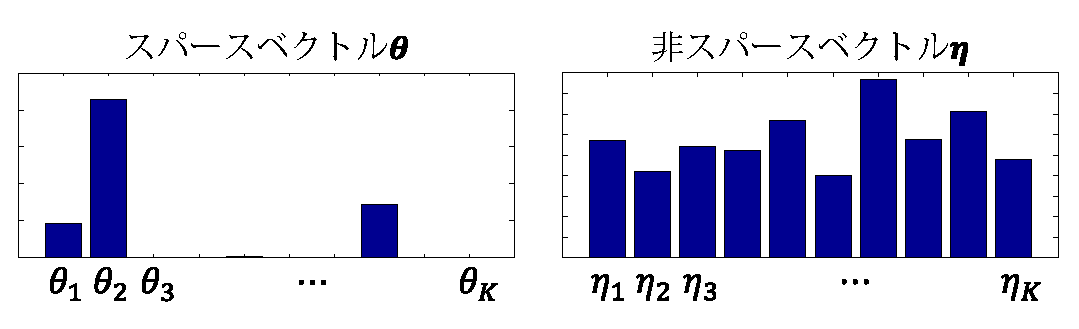
\includegraphics[width=.93\linewidth]{sections/music/sparse}
\caption{$K$次元のスパースベクトル$\bm\theta$と非スパースベクトル$\bm\eta$.
各ベクトルは各次元$k \ (1 \le k \le K)$に対して
$\theta_k \sim \mbox{Gamma}(0.1, 0.1)$,$\eta_k \sim \mbox{Gamma}(10, 10)$としてランダムに生成.
ただし,$\mathbb{E}[\theta_k] = \mathbb{E}[\eta_k] = 1$であることに注意.}
\label{fig:sparse}
\end{figure}

\begin{figure}[t]
\centering
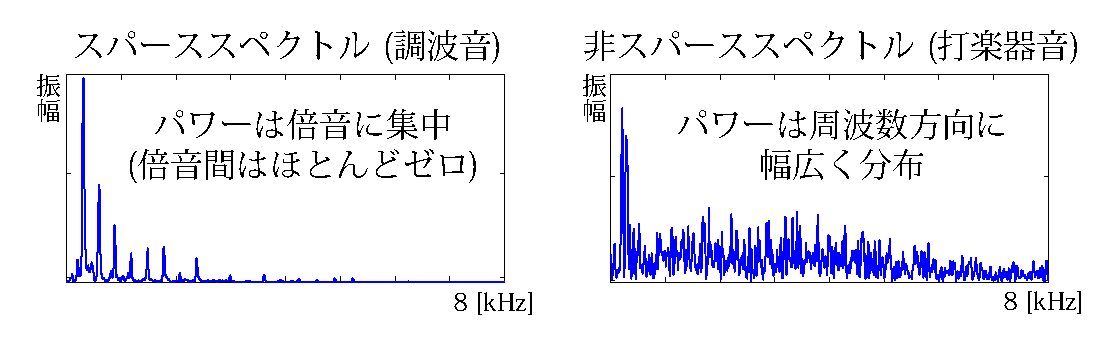
\includegraphics[width=.99\linewidth]{sections/music/sparse_spec}
\caption{調波構造を持つ楽器音(ピアノ)のパワースペクトルと
調波構造を持たない打楽器音(スネアドラム)のパワースペクトル.}
\label{fig:sparse_spec}
\end{figure}

ベクトルや行列がスパースであるとは,
ほとんどの要素がゼロをとる状態を指します(\reffig{fig:sparse}).
一見複雑に思える音楽音響信号も,
高々有限個の楽器音が重なりあってできています.
例えば,あるピアノ曲を考えてみると,
楽曲中に出現する音高は音域や調に依存することから,
ピアノの持つ88種類の音高(鍵盤の個数)の使われやすさに大きな偏りがあります.
また,音楽音響信号の構成要素そのものにもスパース性が存在します.
例えば,調波構造を持つ楽器音は,
倍音周波数付近にパワーが集中しており,
倍音間にはほとんどパワーが存在しません(\reffig{fig:sparse_spec}).
一方,バスドラムやスネアドラムのように,
明確な音高を持たない打楽器音は,周波数方向に幅広くパワーが分布しており,
スパースではありません.
\reffig{fig:sparse}に示すように,適切な確率分布を用いれば,
スパース性を表現することができます.

\subsection{低ランク性}

\begin{figure}[t]
\centering
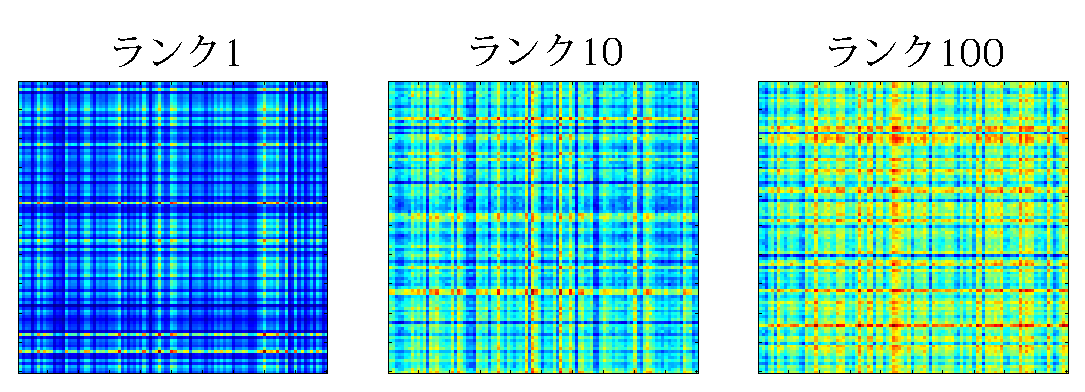
\includegraphics[width=.99\linewidth]{sections/music/low_rank_matrices}
\caption{ランク$K=1,10,100$の行列の例.
各行列$\bm{X}$は,$A_{nk} \sim \mbox{Gamma}(10,10)$および$B_{km} \sim \mbox{Gamma}(10,10)$として
行列$\bm{A} \in \mathbb{R}^{N \times K}$および
$\bm{B} \in \mathbb{R}^{K \times M}$をランダムに生成したあと,$\bm{X}=\bm{A}\bm{B}$として計算.}
\label{fig:low_rank_matrices}
\end{figure}

ある行列$\bm{X} \in \mathbb{R}^{N \times M}$が低ランクであるとは,
$K \ll M, N$として,
\begin{align}
\bm{X} = \bm{A}\bm{B}
\end{align}
となるような
行列$\bm{A} \in \mathbb{R}^{N \times K}$および
$\bm{B} \in \mathbb{R}^{K \times M}$が存在することをいいます.
ここで,$K$はランク(階数)と呼ばれ,
もとの行列$\bm{X}$の行数$M$や列数$N$よりはるかに小さい値をとります.
究極的には,$K=1$である場合に$\bm{X}$はランク1の行列となり,
$\bm{X} = \bm{a}\bm{b}^T$となるようなベクトル$\bm{a} \in \mathbb{R}^{N}$および
$\bm{B} \in \mathbb{R}^{M}$の直積で表現されます.

\begin{figure}[t]
\centering
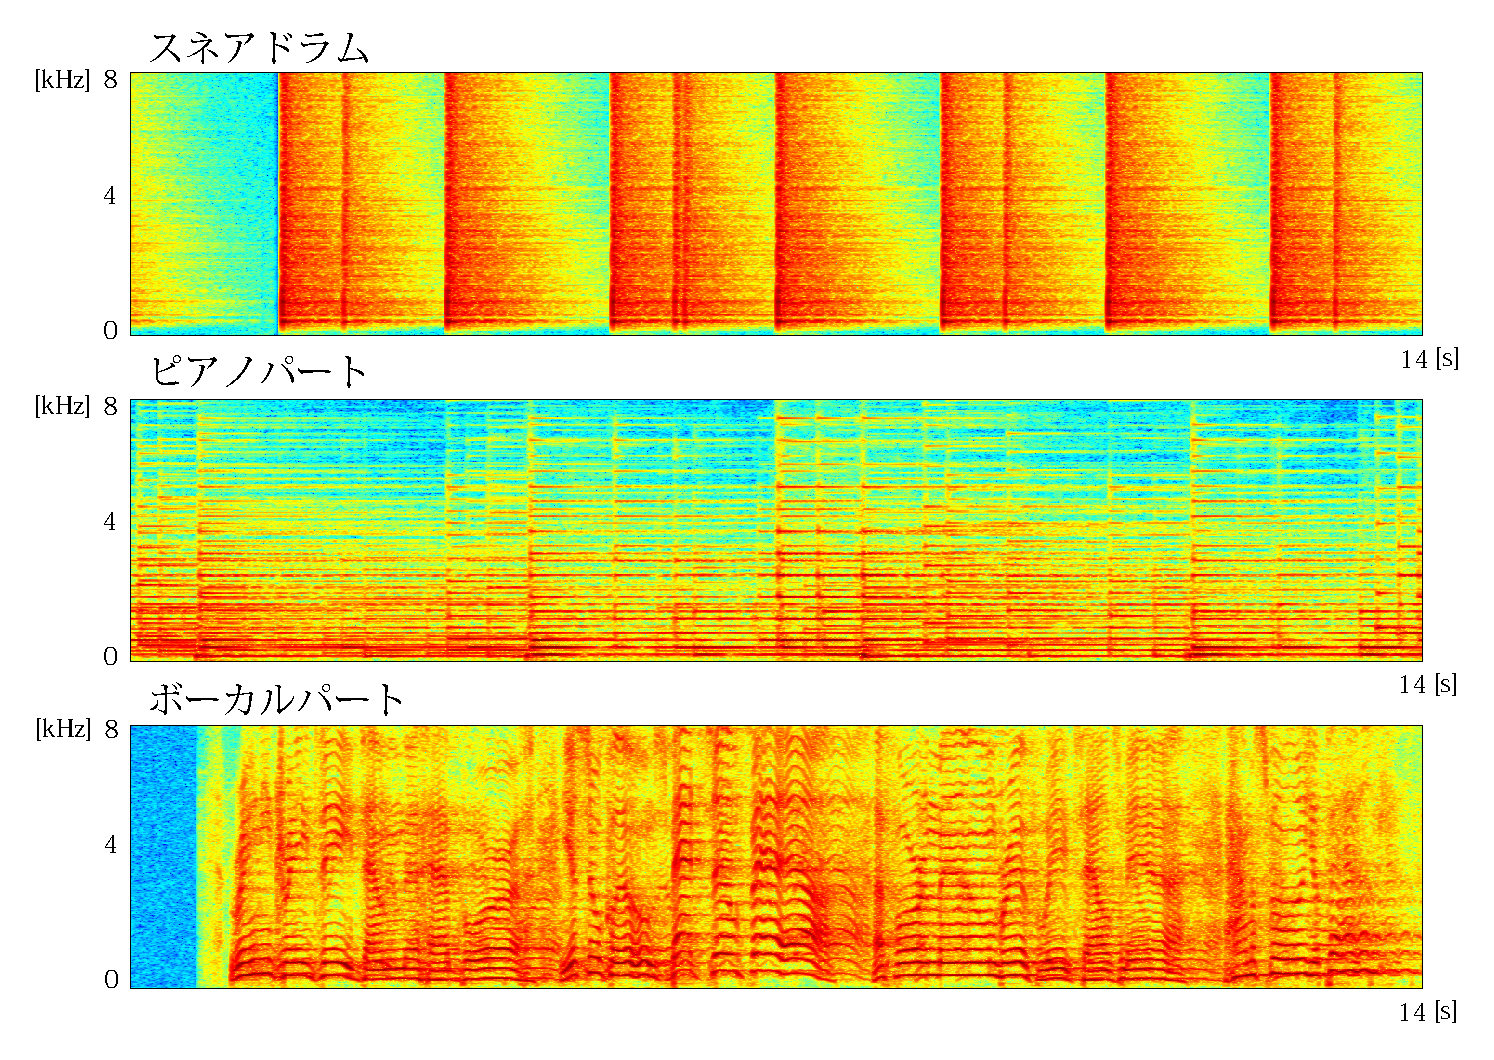
\includegraphics[width=.99\linewidth]{sections/music/low_rank_spectrograms}
\caption{スネアドラム,ピアノパート,ボーカルパートのパワースペクトログラム.
これらをそれぞれ行列とみなしたときに,この順番にランクが増加すると考えられる.
研究コミュニティベースの音源分離コンテストSiSEC 2008\cite{vincent:sisec:2008}において配布されている
開発用データに含まれる楽曲``bearlin roads''を利用.}
\label{fig:low_rank_spectrograms}
\end{figure}

低ランクの行列を可視化してみると,
布地の織り目のような縦横の模様があることに気づきます(\reffig{fig:low_rank_matrices}).
特にランク1の場合,行列を任意の場所で縦方向にスライスしてみると,
抜き出されるベクトルの全体的な形状は一定であり,そのスケールのみが変化することになります
(場所ごとに直径が変化する金太郎あめを想像してください).
行列を任意の場所で横方向にスライスする場合も同じことです.

実際の楽器音のスペクトログラムも,同様の縦横の模様を持っています(\reffig{fig:low_rank_matrices}).
特に,バスドラムやスネアドラムといった打楽器音は,
同じ形状のパワースペクトルが何度も繰り返し出現し,
各発音時刻の後では,パワースペクトルの形状が保たれたまま
音量が徐々に減衰していく現象がみられることから,
低ランクな行列(理想的にはランク1の行列)で近似することはある程度妥当であると考えられます.
ピアノパートは複数の音高の重畳で成り立っているため,
ランク1の行列で近似することは困難なものの,
やはり低ランク構造を持ちそうなことが分かります.
一方,ボーカルパートは,時間方向・周波数方向にパワースペクトルが複雑に変化しているため,
低ランクの行列とはみなすことは困難です.


\subsection{音源分離への応用}
\label{sec:nmf_separation}

NMFでは,基底ベクトル$\bm{w}_k$及び
アクティベーションベクトル$\bm{h}_k$がスパースになりやすい.
一方,同様の行列分解形式$\bm{X} = \bm{W}\bm{H}$を持つ
主成分分析 (Principal Component Analysis: PCA) では,
行列要素は負値をとることが許されている.
従って,\refeq{eqn:x_wh_elem}のように入力を基底の線形和で表現する際に,
基底の加減算による細かな調節が可能となる.
一方,NMFでは,基底の加算しか許されず,
いったんアクティベートされた基底の影響を打ち消すことはできない.
そのため,各基底$\bm{w}_k$が$\bm{x}_n$中の局所的な「パーツ」に対応し,
少数の基底で$\bm{x}_n$を表現する方が都合が良い.
NMFは当初,顔画像(ピクセル値ベクトル)の集合に対して適用され,
目・鼻・口といった顔のパーツ画像に対応する基底ベクトルが得られることが分かった.
このようなパーツに基づく分解表現は,音楽音響信号の分解と相性が良い.
なぜなら,調波音のスペクトルは周波数軸上でスパースであり,
混合音スペクトルは局所的な周波数帯域上のパーツの組み合わせとみなせるからである.

観測信号の複素スペクトログラムを
$\tilde{\bm{X}} = [\tilde{\bm{x}}_1,\cdots,\tilde{\bm{x}}_N] \in \mathbb{C}^{M \times N}$,
$k$番目の音源信号の複素スペクトログラムを
$\tilde{\bm{X}}_k = [\tilde{\bm{x}}_{k1},\cdots,\tilde{\bm{x}}_{kN}] \in \mathbb{C}^{M \times N}$とする.
$M$は周波数ビン数,$N$はフレーム数である.
観測した混合音が$K$個の音源信号の瞬時混合であると仮定すると,以下が成立する.
\begin{align}
 \tilde{\bm{X}} = \sum_{k=1}^{K} \tilde{\bm{X}}_{k}
 \ 
 \left(
 \tilde{\bm{x}}_n = \sum_{k=1}^{K} \tilde{\bm{x}}_{kn}
 \right)
 \label{eqn:s}
\end{align}

観測変数$\tilde{\bm{X}}$を潜在変数$\tilde{\bm{X}}_k$に分解する問題は不良設定であるので,
$\tilde{\bm{X}}_k$に対応する
パワースペクトログラム$\bm{X}_k = [\bm{x}_{k1},\cdots,\bm{x}_{kN}] 
\in \mathbb{R}_+^{M \times N}$ $(x_{knm} = |\tilde{x}_{knm}|^2)$は,
ランク1行列$\bm{Y}_k = [\bm{y}_{k1},\cdots,\bm{y}_{kN}] \in \mathbb{R}_+^{M \times N}$で
近似する(\reffig{fig:nmf}).
\begin{align}
 \bm{X}_k \approx \bm{w}_k \bm{h}_k^T \overset{\mbox{\tiny def}}{=} \bm{Y}_k
 \label{eqn:rank1}
\end{align}
すなわち,$\bm{Y}_k$の任意のフレーム$n$におけるパワースペクトル$\bm{y}_{kn}$は
基底スペクトル$\bm{w}_k \in \mathbb{R}^{M}$を
重み$h_{kn}$でスケーリングするだけで得られるという仮定をおいた($\bm{y}_{kn} = h_{kn} \bm{w}_k$).
%本来,調波構造中の倍音の相対強度は時変であるが,
%実際のスペクトル$\bm{X}_k$に対する近似モデルとしては有効に機能する.

\begin{figure}[t]
\centering
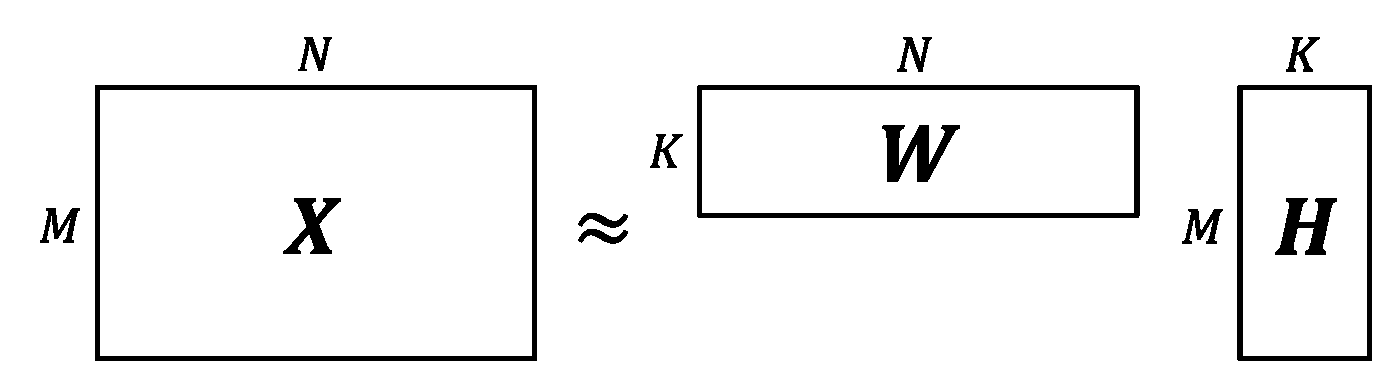
\includegraphics[width=.99\linewidth]{sections/music/nmf}
\caption{パワースペクトログラムに対する
ISダイバージェンスに基づく非負値行列分解 (IS-NMF) の適用結果.}
\label{fig:nmf}
\end{figure}

まず,潜在変数$\tilde{\bm{x}}_{kn}$が
$\bm{y}_{kn}$で定まる対角共分散行列を持つ複素ガウス分布に従うことを仮定する.
\begin{align}
 \tilde{\bm{x}}_{kn} \sim \mathcal{N}_c(\bm{0}, \mbox{diag}(\bm{y}_{kn}))
 \label{eqn:is_s_k_p}
\end{align}
ただし,$\mbox{diag}(\bm\eta)$はベクトル$\bm\eta$を対角成分に持つ対角行列を表す.
\refeq{eqn:s}に着目すると,
複素ガウス分布の再生性から
\begin{align}
 \tilde{\bm{x}}_n \sim \mathcal{N}_c(\bm{0}, \mbox{diag}(\bm{y}_n))
  \label{eqn:is_s_p}
\end{align}
を得る.ただし,$\bm{y}_n = \sum_k \bm{y}_{kn}$である.
従って,$x_{nm}=|\tilde{x}_{nm}|^2$は指数分布に従うことが分かる.
\begin{align}
 x_{nm} \sim \mbox{Exponential}(y_{nm})
 \label{eqn:is_p}
\end{align}
ここで,\refeq{eqn:is_s_p}の対数をとって符号反転させると,
\refeq{eqn:nmf_is}と定数項を除いて等しい.
従って,\refeq{eqn:is_s_p}の最大化(最尤推定)は
\refeq{eqn:nmf_is}の最小化と等価であり,
IS-NMFの適用が適切であると分かる.

最終的に,\refeq{eqn:is_s_k_p}及び\refeq{eqn:is_s_p}に着目すると,
$\tilde{\bm{x}}_n$が与えられたときの
$\tilde{\bm{x}}_{kn}$の事後分布は複素ガウス分布になることが分かり,
その平均と分散は
\begin{align}
 &
 \mathbb{E}[\tilde{\bm{x}}_{kn}|\tilde{\bm{x}}_{n}] 
 = \mbox{diag}(\bm{y}_{kn}) \mbox{diag}(\bm{y}_n)^{-1} \tilde{\bm{x}}_{n}
 \label{eqn:s_exp}
 \\
 &
 \mathbb{V}[\tilde{\bm{x}}_{kn}|\tilde{\bm{x}}_{n}] 
 = \mbox{diag}(\bm{y}_{kn}) 
 \nonumber\\
 & \ \ \ \ \
 - \mbox{diag}(\bm{y}_{kn}) \mbox{diag}(\bm{y}_n)^{-1} \mbox{diag}(\bm{y}_{kn})
 \label{eqn:s_var}
\end{align}
で与えられる.
この処理はウィナーフィルタリングと呼ばれ,
$\tilde{\bm{X}}_k$の位相は$\tilde{\bm{X}}$の位相と同一であるという仮定が置かれている.
最後に,逆フーリエ変換を用いて,
$\mathbb{E}[\tilde{\bm{X}}_k|\tilde{\bm{X}}]$から
$k$番目の音源信号を復元することができる.

\begin{figure}[t]
\centering
\includegraphics[width=.98\linewidth]{sections/music/nmf_samples}
\caption{異なる基底数$K$に対するIS-NMFの結果.}
\label{fig:nmf_samples}
\end{figure}

基底数$K$を変化させながらIS-NMFを適用した結果を\reffig{fig:nmf_samples}に示す.
$K$が小さすぎると近似が荒く,
$K$を大きくしすぎると物理的な意味を持たない極めて局所的な基底ばかりになる.
このことから,基底数$K$を適切に定める重要性が分かる.

実際には,性質の良くない局所解に陥りやすいIS-NMFの代わりに
KL-NMFが利用される場合が多い.
このとき,$\bm{X}$や$\bm{X}_k$は
振幅スペクトログラムとするのが一般的である($x_{knm} = |\tilde{x}_{knm}|$).

まず,潜在変数$x_{knm}$が$y_{knm}$で定まるポアソン分布に従うことを仮定する.
\begin{align}
 x_{knm} \sim \mbox{Poisson}(y_{knm})
 \label{eqn:kl_s_k_p}
\end{align}
ここで,複数の音源信号の重畳における振幅スペクトルの加法性を仮定すると
(実際には成立しないことに注意),ポアソン分布の再生性から
\begin{align}
 x_{nm} \sim \mbox{Poisson}(y_{nm})
 \label{eqn:kl_s_p}
\end{align}
を得る.
ここで,\refeq{eqn:kl_s_p}の対数をとって符号反転させると,
\refeq{eqn:nmf_kl}と定数項を除いて等しい.
従って,\refeq{eqn:kl_s_p}の最大化(最尤推定)は
\refeq{eqn:nmf_kl}の最小化と等価である.


\subsection{音源分離への応用}
\label{sec:mf}

\refeq{eqn:s}を満たすように,
$\tilde{\bm{x}}_n$を
$\{\tilde{\bm{x}}_{kn}\}_{k=1}^K$の和に分解したい.
まず,潜在変数$\tilde{\bm{x}}_{kn}$が
共分散行列$\bm{Y}_{kn}$を持つ複素ガウス分布に従うことを仮定する.
\begin{align}
 \tilde{\bm{x}}_{kn} \sim \mathcal{N}_c(\bm{0}, \bm{Y}_{kn})
 \label{eqn:ld_s_k_p}
\end{align}
ここで,\refeq{eqn:is_s_k_p}のように共分散行列を対角行列に限定しないことで,
周波数ビン間の相関を考慮している.
\refeq{eqn:s}と複素ガウス分布の再生性から
\begin{align}
 \tilde{\bm{x}}_n \sim \mathcal{N}_c(\bm{0}, \bm{Y}_n)
  \label{eqn:ld_s_p}
\end{align}
を得る.ただし,$\bm{Y}_n = \sum_k \bm{Y}_{kn}$である.
ここで,\refeq{eqn:ld_s_p}の対数をとって符号反転させると,
\refeq{eqn:psdtf_ld}と定数項を除いて等しい.
従って,\refeq{eqn:ld_s_p}の最大化は
\refeq{eqn:psdtf_ld}の最小化と等価であり,
LD-PSDTFを用いて$\bm{Y}_n$や$\bm{Y}_{kn}$を求めることができる.

最終的に,\refeq{eqn:ld_s_k_p}, (\ref{eqn:ld_s_p})から,
$\tilde{\bm{x}}_n$が与えられたときの
$\tilde{\bm{x}}_{kn}$の事後分布は複素ガウス分布になることが分かり,
その平均と分散は次式となる.
\begin{align}
 &\!\!\!\!\!\!\!\!
 \mathbb{E}[\tilde{\bm{x}}_{kn}|\tilde{\bm{x}}_n] 
 =
 \bm{Y}_{kn} \bm{Y}_n^{-1} \tilde{\bm{x}}_n
 \label{eqn:e_xn}
 \\
 &\!\!\!\!\!\!\!\!
 \mathbb{V}[\tilde{\bm{x}}_{kn}|\tilde{\bm{x}}_n] 
 =  
 \bm{Y}_{kn} - \bm{Y}_{kn} \bm{Y}_n^{-1} \bm{Y}_{kn}
 \label{eqn:v_xn}
\end{align}
ここで,\refeq{eqn:s_exp}とは異なり,
$\tilde{\bm{X}}_k$の位相は$\tilde{\bm{X}}$の位相とは異なる点に注意する.
IS-NMFのように各周波数ビン$n,m$ごとではなく,
各フレーム$n$ごとに一挙に分離を行うことで,
周波数ビン間の相関を考慮しながら高品質な分離が可能となる.

\begin{algorithm}[t]
\caption{LD-PSDTFの最尤推定}         
\label{ld-psdtf-ml}
\begin{algorithmic}[1]
\Require テンソル$\bm{X} \in \mathbb{C}^{M \times M \times N}$, 基底数$K$
\State 基底テンソル$\bm{W} \in \mathbb{C}^{M \times M \times K}$をランダムに初期化
\State 非負値行列$\bm{H} \in \mathbb{R}_+^{M \times K}$をランダムに初期化
\While{not converged}
\State $\bm{P}_k = \sum_{n=1}^{N} h_{kn} \bm{Y}_n^{-1}$
\State $\bm{Q}_k = \sum_{n=1}^{N} h_{kn} \bm{Y}_n^{-1} \bm{X}_n \bm{Y}_n^{-1}$
\State コレスキー分解$\bm{Q}_k = \bm{L}_k \bm{L}_k^T$
\State $\bm{W}_k 
 \gets
 \bm{W}_k \bm{L}_k(\bm{L}_k^T \bm{W}_k \bm{P}_k \bm{W}_k \bm{L}_k)^{-\frac{1}{2}}\bm{L}_k^T \bm{W}_k$
\State  $h_{kn} \gets h_{kn}
 \left(\frac{\mbox{tr}\!\left(\bm{Y}_n^{-1} \bm{W}_k \bm{Y}_n^{-1} \bm{X}_n\right)}
            {\mbox{tr}\!\left(\bm{Y}_n^{-1} \bm{W}_k \right)}\right)^{\frac{1}{2}}$
\EndWhile\\
{\bf Return} 基底テンソル$\bm{W}$,非負値行列$\bm{H}$
\end{algorithmic}
\end{algorithm}

\subsection{確率モデルの最尤推定としての定式化}

文献\cite{yoshii:ismir:2013,yoshii:icml:2013}において,
NMFと同様にガンマ過程を用いて基底数を$K \rightarrow \infty$とした
ノンパラメトリックベイズモデルが提案されている.
今後の課題として,vN-PSDTFに対する乗法更新則の導出や計算量の削減が挙げられる.



\section{楽器パートの分離}

\subsection{歌声・伴奏音の分離}

最後に,スパース性に基づいて音楽音響信号を楽器種別に分離する技術を紹介する.
ロバスト主成分分析 (RPCA) は,入力行列$\bm{X}$を
低ランク行列$\bm{L}$とスパース行列$\bm{S}$の和に分解する.
具体的には,$\bm{X} = \bm{L} + \bm{S}$を満たすという制約のもとで,
以下で定義される最適化問題を解く.
\begin{align}
 \mbox{minimize} \ \|\bm{L}\|_* +\lambda \|\bm{S}\|_1
\end{align}
ここで,$\|\cdot\|_*$,$\|\cdot\|_1$はそれぞれ核ノルム,L1ノルムである.
厳密ではないが拡張ラグランジュ法に基づく効率的な解法を{\bf Algorithm \ref{rpca}}に示す.
\refsec{sec:introduction}で議論したとおり,
混合音スペクトログラムを$\bm{X}$として与えると,
伴奏音スペクトログラム$\bm{L}$と歌声スペクトログラム$\bm{S}$が得られる.
また,メディアンフィルタを時間方向・周波数方向に適用することで
調波音・打楽器音を分離すること (Harmonic/Percussive Source Separation: HPSS) 
も可能である\cite{fitzgerald:dafx:2010}.
これらの技術による分離結果を\reffig{fig:separation}に示す.

\begin{algorithm}[t]
\caption{Inexact ALMに基づくRPCA}
\label{rpca}                          
\begin{algorithmic}[1]
\Require 入力行列$\bm{X} \in \mathbb{R}^{M \times N}$,重み係数$\lambda$
\State 初期化:$\bm{Y} = \bm{X} / \max(\|\bm{X}\|_2, \lambda^{-1}\|\bm{X}\|_\infty) \in \mathbb{R}^{M \times N}$
\State 初期化:$\bm{S} = \bm{0} \in \mathbb{R}^{M \times N}$
\State 初期化:$\mu > 0$ ({\it e.g.}, $\mu = 1.25 / \|\bm{X}\|_2 $)
\State 初期化:$\rho > 1$ ({\it e.g.}, $\rho = 1.5$)
\While{not converged}
\State $[\bm{U}, \bm\Sigma, \bm{V}] = \mbox{SVD}(\bm{X} - \bm{S} + \mu^{-1} \bm{Y})$
\State $\bm{L} \gets \bm{U} \mathcal{F}_{\mu^{-1}}(\bm\Sigma) \bm{V}^T$
\State $\bm{S} \gets \mathcal{F}_{\lambda\mu^{-1}}(\bm{X} - \bm{L} + \mu^{-1} \bm{Y})$
\State $\bm{Y} \gets \bm{Y} + \mu (\bm{X} - \bm{L} - \bm{S})$
%\If {$\mu\|\bm{S} - \bm{S}_{\mbox{\scriptsize old}}\|_F/\|\bm{X}\|_F < \epsilon$}
\State $\mu \gets \rho \mu$
%\EndIf
\EndWhile
\\
{\bf Return} 低ランク行列$\bm{L}$,
スパース行列$\bm{S} \in \mathbb{R}^{M \times N}$
\end{algorithmic}
*$\mathcal{F}_\epsilon[x] 
= x - \epsilon \ (\mbox{if} \ x > \epsilon), 
  x + \epsilon \ (\mbox{if} \ x < -\epsilon), 
  0 \ (\mbox{otherwise})$
\end{algorithm}

\subsection{調波音・非調和音の分離}

HPSSのいくつかの手法を紹介.

\subsection{音色に基づく分離}

ソースフィルタモデル

\section{おわりに}

本稿では,スパース性に基づく音楽音響信号分解技術として,
非負値行列分解 (NMF),半正定値テンソル分解 (PSDTF),
ロバスト主成分分析 (RPCA),調波・打楽器分離音 (HPSS) を紹介した.
これらは音声情報処理分野の影響を受けながら,
音楽情報処理分野で独自の発展を遂げている.
例えば,NMF(音響モデル)はソース・フィルタ型の楽器音モデルや,
楽譜の生成モデル(言語モデル)と統合する試みが進んでいる.
本稿が読者の理解の一助になれば幸いである.

\begin{figure}[t]
\centering
\includegraphics[width=.99\linewidth]{sections/music/separation}
\caption{音楽音響信号に対するRPCA・HPSSの適用結果.}
\label{fig:separation}
\end{figure}

%% 文献
%\bibliographystyle{unsrt}
%\bibliography{yoshii,yoshii-nmf,yoshii-lpc}

\begin{thebibliography}{10}

\bibitem{lee:nature:1999}
D. D. Lee and H. S. Seung, 
\newblock ``Learning the parts of objects by non-negative matrix factorization,'' 
\newblock {\em Nature}, {\bf 401}, 788--791 (1999).

\bibitem{fevotte:neco:2009}
C.‾{F\'{e}votte}, N.‾Bertin, and J.-L. Durrieu,
\newblock ``Nonnegative matrix factorization with the {I}takura-{S}aito
  divergence: {W}ith application to music analysis,''
\newblock {\em Neural Computation}, {\bf 21(3)}, 793--830 (2009).

\bibitem{hoffman:icml:2010}
M.‾Hoffman, D.‾Blei, and P.‾Cook,
\newblock ``{B}ayesian nonparametric matrix factorization for recorded music,''
\newblock {\em ICML}, 439--446 (2010).

\bibitem{yoshii:icml:2013}
K.‾Yoshii, R.‾Tomioka, D.‾Mochihashi, and M.‾Goto,
\newblock ``Infinite positive semidefinite tensor factorization for source
  separation of mixture signals,''
\newblock {\em ICML}, 576--584 (2013).

\bibitem{yoshii:ismir:2013}
K.‾Yoshii, R.‾Tomioka, D.‾Mochihashi, and M.‾Goto,
\newblock ``Beyond NMF: Time-domain audio source separation without phase
  reconstruction,''
\newblock {\em ISMIR}, 369--374 (2013).

\bibitem{lin:mp:2010}
Z.‾Lin, M.‾Chen, and Y.‾Ma,
\newblock ``The augmented {L}agrange multiplier method for exact recovery of
  corrupted low-rank matrices,''
\newblock {\em Math. Prog.} (2010).

\bibitem{fitzgerald:dafx:2010}
D.‾FitzGerald,
\newblock ``Harmonic/percussive separation using median filtering,''
\newblock {\em DAFx} (2010).

\bibitem{smaragdis:waspaa:2003}
P.‾Smaragdis and J.‾C. Brown,
\newblock ``Non-negative matrix factorization for polyphonic music transcription,''
\newblock {\em WASPAA}, 177--180 (2003).

\bibitem{kameoka:asjj:2012}
亀岡弘和,
\newblock ``非負値行列因子分解の音響信号処理への応用,''
\newblock {\em 日本音響学会誌}, 68(11), 559--565 (2012).

\bibitem{sawada:ieee:2013}
H.‾Sawada, H.‾Kameoka, S.‾Araki, and N.‾Ueda,
\newblock ``Multichannel extensions of non-negative matrix factorization with complex-valued data,''
\newblock {\em IEEE Trans. TASLP}, {\bf 21(5)}, 971--982 (2013).

\bibitem{kulis:jmlr:2009}
B.‾Kulis, M.‾Sustik, and I.‾Dhillon,
\newblock ``Low-rank kernel learning with {B}regman matrix divergences,''
\newblock {\em JMLR}, {\bf 10}, 341--376 (2009).

\end{thebibliography}



%\section{ソース・フィルタ分解}

%\section{調波音・打楽器音分離}

%\section{時間領域分解}

%また,構成要素のスパース性に着目することで,
%市販CDのように複雑な音楽音響信号に対しても,
%歌声・伴奏音を分離したり,調波音・打楽器音を分離することができる.
%音色や音高のバリエーションに富む歌声を含む音楽音響信号は,
%NMFのように少数の基底の線形和で表現することは難しい.
%一方,ロバスト主成分分析 (Robust Principal Component Analysis: RPCA)\cite{lin:mp:2010}
%を用いると,線形和で表現可能な低ランクな伴奏音成分と,
%外れ値とみなせるスパースな歌声成分とに分離可能である.
%また,時間・周波数平面において,
%調波構造を持つ楽器音は周波数方向にスパースであり,
%減衰が早い打楽器音は時間方向にスパースである.
%従って,周波数・時間方向にそれぞれメディアンフィルタを適用すれば,
%外れ値となる調波音・打楽器音をそれぞれ抑制することができる\cite{fitzgerald:dafx:2010}.

